%%%%%%%%%%%%%%%%%%%%%%%%%%%%%%%%%%%%%%%%%%%%%%%%%%%%%%%%%%%%%%%%%%%%%%%%%%%%
%
%%%%%%%%%%%%%%%%%%%%%%%%%%%%%%%%%%%%%%%%%%%%%%%%%%%%%%%%%%%%%%%%%%%%%%%%%%%%
%
% IMPORTANT NOTE:
%
% SUPPORTING INFORMATION DOCUMENTATION IS NOT COPYEDITED BEFORE PUBLICATION.
%
%%%%%%%%%%%%%%%%%%%%%%%%%%%%%%%%%%%%%%%%%%%%%%%%%%%%%%%%%%%%%%%%%%%%%%%%%%%%

\documentclass[draft,grl]{agutexSI2019}

\usepackage{url} %this package should fix any errors with URLs in refs.
\usepackage{lineno}
 \usepackage{graphicx}
 \usepackage{rotating}
\usepackage{minted}
%\usepackage{makecell}
\usepackage{xr}
%\usepackage{subfiles}
\usepackage{float}
%\usepackage{caption}
\usepackage{xr}
\makeatletter

%\DeclareCaptionFormat{cancaption}{#1#2#3\par} % Normal format actually
%\DeclareCaptionLabelFormat{cancaptionlabel}{#1 S#2}

%
\usepackage[inline]{trackchanges} %for better track changes. finalnew option will compile document with changes incorporated.
\usepackage{soul}

\linenumbers

%%%%%%%%%%%%%%%%%%%%%%%%%%%%%%%%%%%%%%%%%%%%%%%%%%%%%%%%%%%%%%%%%%%%%%%%%
%
%  SUPPORTING INFORMATION TEMPLATE
%
%% ------------------------------------------------------------------------ %%
%
%
%Please use this template when formatting and submitting your Supporting Information.

%This template serves as both a “table of contents” for the supporting information for your article and as a summary of files.
%
%
%
%USING THIS TEMPLATE
%
%***All references should be included in the reference list of the main paper so that they can be indexed, linked, and counted as citations.  The reference section does not count toward length limits.

%

%
%  Uncomment the following command to allow illustrations to print
%   when using Draft:
 \setkeys{Gin}{draft=false}
%

% Author names in capital letters:
\authorrunninghead{ZARAKAS ET AL.}

%% Corresponding Author:
\authoraddr{Corresponding author: Claire M. Zarakas, czarakas@uw.edu}

\begin{document}

\title{Supporting Information for ``Land Processes Can Substantially Impact the Mean Climate State''}

%DOI: 10.1002/%insert paper number here%


\authors{Claire M. Zarakas\affil{1} , 
Daniel Kennedy\affil{3}, 
Katherine Dagon\affil{3}, 
David M. Lawrence\affil{3}, 
Amy Liu\affil{1}, 
Gordon Bonan\affil{3}, 
Charles Koven\affil{4},
Danica Lombardozzi\affil{3},
and Abigail L. S. Swann\affil{1,2}}

\affiliation{1}{University of Washington, Department of Atmospheric Sciences}
\affiliation{2}{University of Washington, Department of Biology}
\affiliation{3}{National Center for Atmospheric Research}
\affiliation{4}{Lawrence Berkeley National Laboratory}

%% ------------------------------------------------------------------------ %%

\begin{article}

\noindent\textbf{Contents of this file}
%%%Remove or add items as needed%%%
\begin{enumerate}
\item Text S1 to S3
\item Figures S1 to Sx
\item Tables S1 to S3
%if Tables are larger than 1 page, upload as separate excel file
\end{enumerate}
%\clearpage{}

%Delete all unused file types below. Copy/paste for multiples of each file type as needed.
%\noindent\textbf{Text S1.}

\noindent\textbf{Text S1: Calculating the pattern of warming due to a doubling of CO$_2$}

\noindent\textbf{Text S2: Robustness testing for disentangling different land surface properties’ contributions to observed temperature changes}

\noindent\textbf{Text S3: Calculating emergent changes in land surface properties}
We calculated the emergent changes in $r_s$ and $r_a$ by inverting the equations for sensible heat flux and latent heat flux (L).  S=($\rho C_p (T_s-T_a))/r_a$  and L=($\rho \lambda(q^* (T_s)-q_a))/(r_a+r_s )$, where $\rho$ is the air density at the lowest atmospheric level, $T_a$ is the air temperature at the lowest atmospheric level, $q_a$ is the specific humidity at the lowest atmospheric level, $T_s$ is land surface skin temperature, and $q^* (T_s)$is the saturated specific humidity at $T_s$. $C_p$ and $\lambda$ are constants, the specific heat of X and the latent heat of vaporization, respectively. We verified our derived changes in $\alpha$, $r_s$, and $r_a$ by demonstrating that they yielded accurate reconstructions of temperature changes in the offline land-only PPE using the two-resistance method (TRM; Rigden and Li 2017), described in Supporting Information X.However, the TRM is ill-suited for attributing quantifying how muchthe  changes in $\alpha$, $r_s$, and $r_a$ drive coupled temperature changes to changes in $\alpha$, $r_s$, and $r_a$ because it combines all temperature changes from atmospheric feedbacks into one term (due to change in Ta), and cannot distinguish the extent to which Ta changes are driven by changes in $\alpha$, $r_s$, and $r_a$.
%Type or paste text here. This should be additional explanatory text, such as: extended descriptions of results, full details of models, extended lists of acknowledgements etc.  It should not be additional discussion, analysis, interpretation or critique. It should not be an additional scientific experiment or paper.
%
%Repeat for any additional Supporting Text
% Note that ALL references in this supporting information file must also be referenced in the primary manuscript
% if you get an error about newblock being undefined, uncomment this line:
%\newcommand{\newblock}{}
%\bibliography{PPE_refs.bib} 
\end{article}


%Reference citation instructions and examples:
%
% Please use ONLY \cite and \citeA for reference citations.
% \cite for parenthetical references
% ...as shown in recent studies (Simpson et al., 2019)
% \citeA for in-text citations
% ...Simpson et al (2019) have shown...
% DO NOT use other cite commands (e.g., \citet, \citep, \citeyear, \nocite, \citealp, etc.).
%
%
%...as shown by \citeA{jskilby}.
%...as shown by \citeA{lewin76}, \citeA{carson86}, \citeA{bartoldy02}, and \citeA{rinaldi03}.
%...has been shown \cite<e.g.,>{jskilbye}.
%...has been shown \cite{lewin76,carson86,bartoldy02,rinaldi03}.
%...has been shown \cite{lewin76,carson86,bartoldy02,rinaldi03}.
%
% apacite uses < > for prenotes, not [ ]
% DO NOT use other cite commands (e.g., \citet, \citep, \citeyear, \nocite, \citealp, etc.).
%

%% ------------------------------------------------------------------------ %%

%\clearpage


%  FIGURES
\begin{figure}[htb!]
 \noindent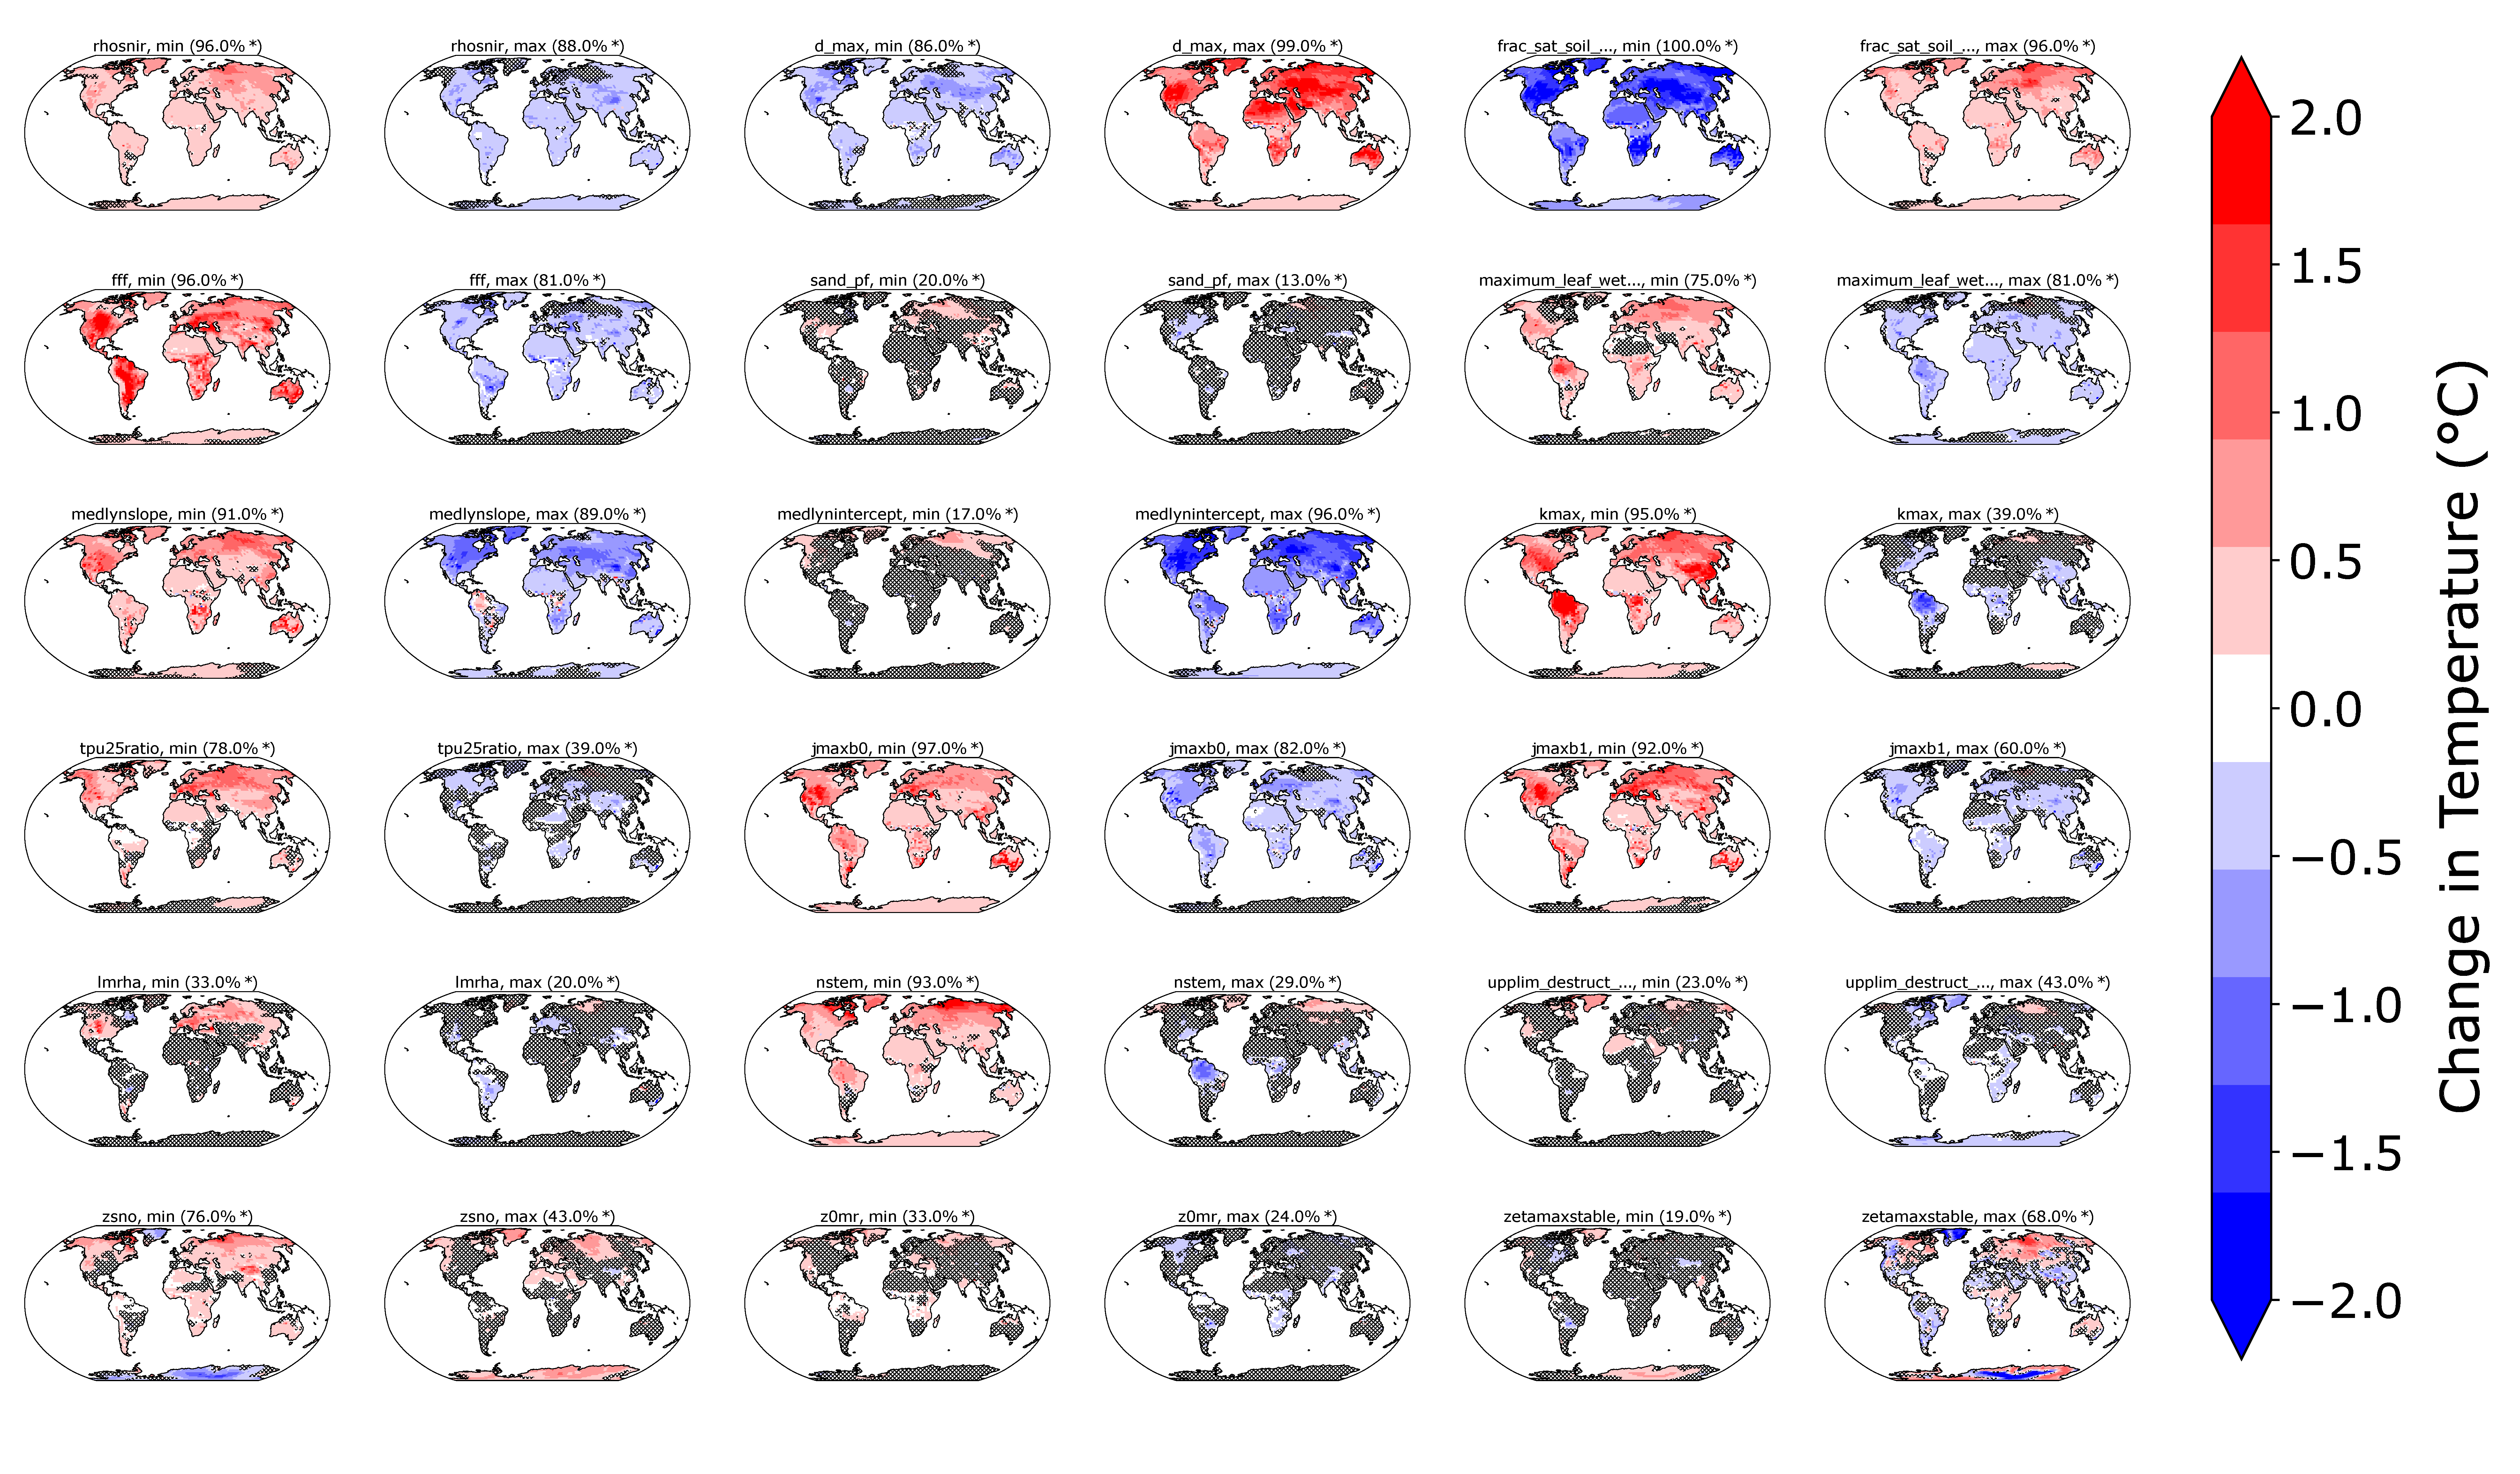
\includegraphics[width=\textwidth]{writing/figs/Figure_S1.pdf}
\caption{Maps of annual mean land temperature changes for each ensemble member, compared to the reference case with default parameterizations. Hatching indicates regions where the temperature change was insignificant at the 0.05 significance level. The percentage of land with statistically significant temperature changes is shown in parentheses, and * indicates field significance. For each grid cell, we performed a two-tailed Student’s t-test to test whether the ensemble member mean (standard deviation calculated from the distribution from interannual variability in the ensemble member mean) was different from the default mean (standard deviation calculated from the distribution from interannual variability in the default mean). We test for field significance using Walker’s test.}
\label{fig:supp_coupled_Ts_land_maps}
\end{figure}

\begin{figure}[htb!]
\noindent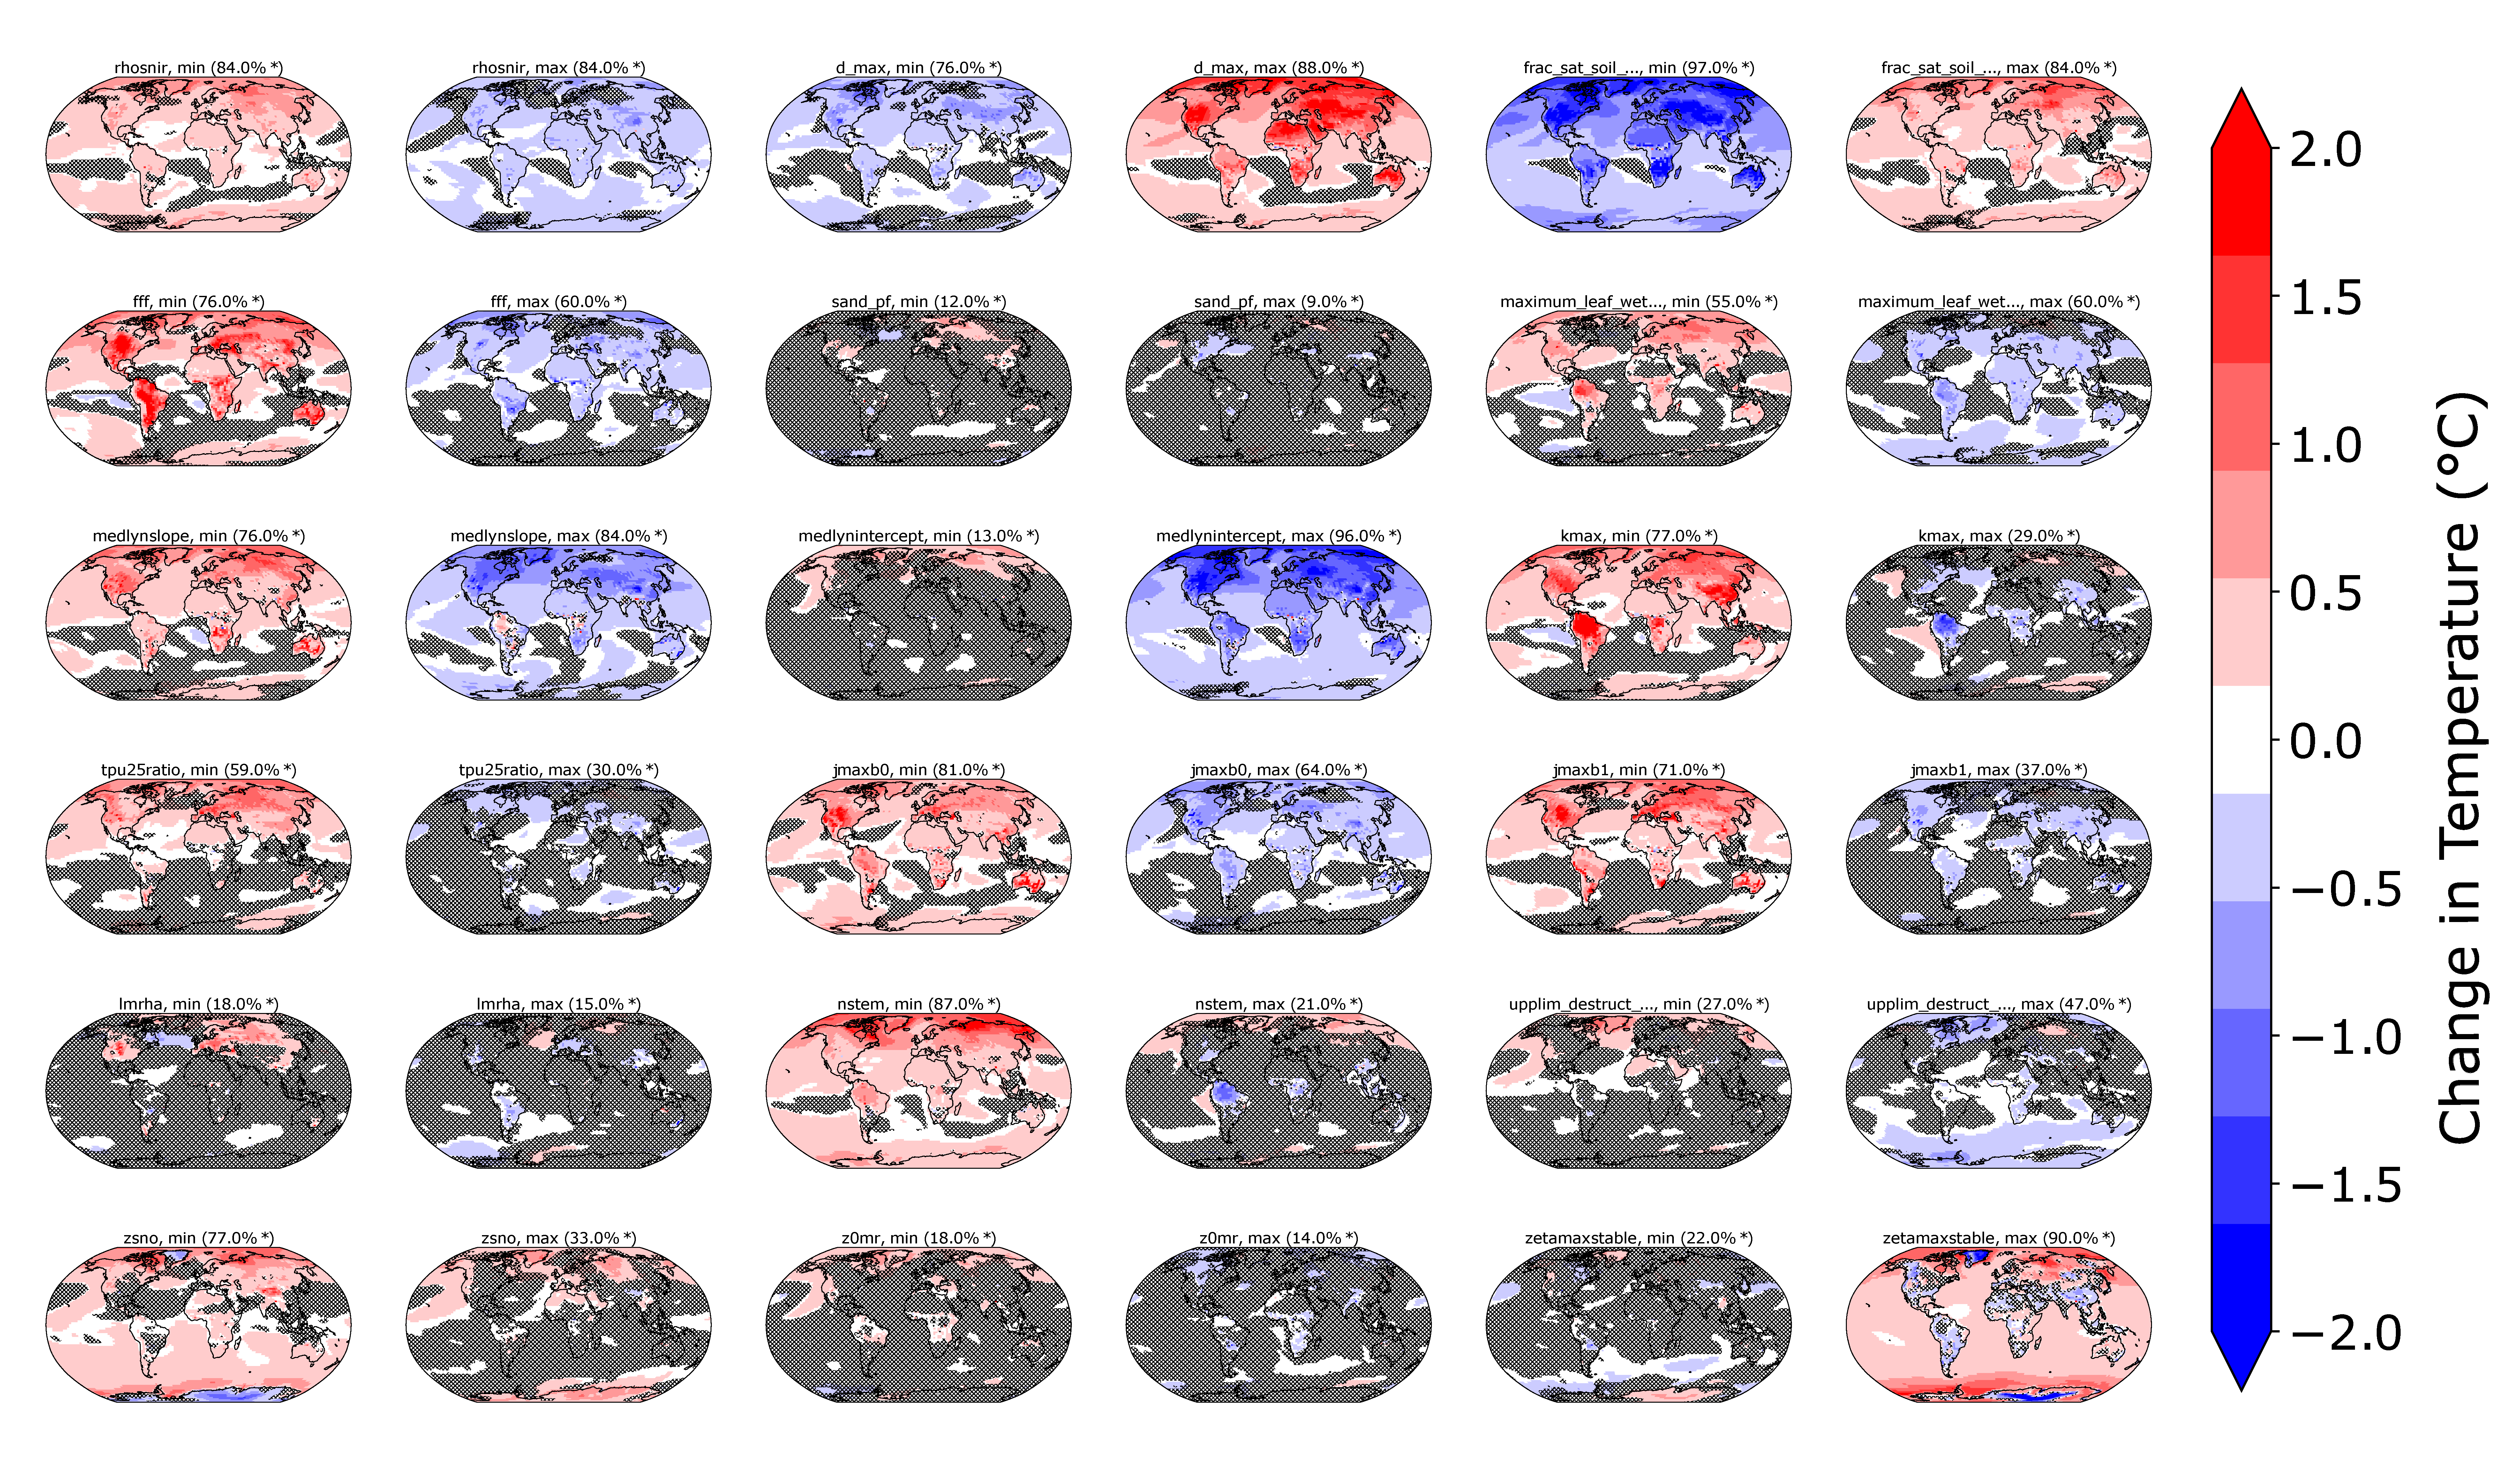
\includegraphics[width=\textwidth]{writing/figs/Figure_S2.pdf}
\caption{Maps of annual mean temperature changes for each ensemble member, including both land and ocean. Hatching and significance testing is as in Figure S1, but the title indicates the total percentage of the Earth surface (including land and ocean) with statistically significant temperature changes.}
\label{fig:supp_coupled_Ts_land_and_ocean_maps}
\end{figure}

\begin{figure}[htb!]
\noindent\includegraphics[width=\textwidth]{writing/figs/Figure_S3.pdf}
\caption{Correlation between the change in annual mean land temperature and annual mean global temperature (including both land and ocean). Colors indicate parameter category as in Figures 1 and 3. Because the parameter \mintinline{Fortran}{zetamaxstable} is an outlier in our PPE, it is denoted as the filled purple point.}
\label{fig:supp_coupled_Ts_land_vs_ocean_maps}
\end{figure}

\begin{figure}[htb!]
\noindent\includegraphics[width=\textwidth]{writing/figs/Figure_S_TSKIN_EOF_summary.pdf}
\caption{EOF analysis of changes in land surface temperature across the PPE. }
\label{fig:supp_EOF_analysis_Temp}
\end{figure}

\begin{figure}[htb!]
\noindent\includegraphics[width=\textwidth]{writing/figs/Figure_S_PRECT_EOF_summary.pdf}
\caption{EOF analysis of changes in land precipitation across the PPE.}
\label{fig:supp_EOF_analysis_Precip}
\end{figure}

\begin{figure}[htb!]
\noindent\includegraphics[width=\textwidth]{writing/figs/Figure_S_Correlation_between_EOFs_and_global_mean_changes.pdf}
\caption{Correlation between leading EOFs of annual average land and temperature changes and global mean annual average land temperature and precipitation changes across the PPE. Ensemble members are colored by parameter category, as in Figure 1.}
\label{fig:supp_EOF_globalmetric_correlation}
\end{figure}

\begin{figure}[htb!]
\noindent\includegraphics[width=\textwidth]{writing/figs/placeholder.pdf}
\caption{S5 Correlation between change in EF and temperature and precipitation EOFs}
\label{fig:supp_EF_EOF_correlation}
\end{figure}


\begin{figure}[htb!]
\noindent\includegraphics[width=\textwidth]{writing/figs/FigureS6.png}
\caption{S6 Rankings of parameters with the largest global mean land-only temperature change. Parameter rankings are based on the output from the land-only CLM5-PPE.}
\label{fig:supp_param_rankings}
\end{figure}

\begin{figure}[htb!]
\noindent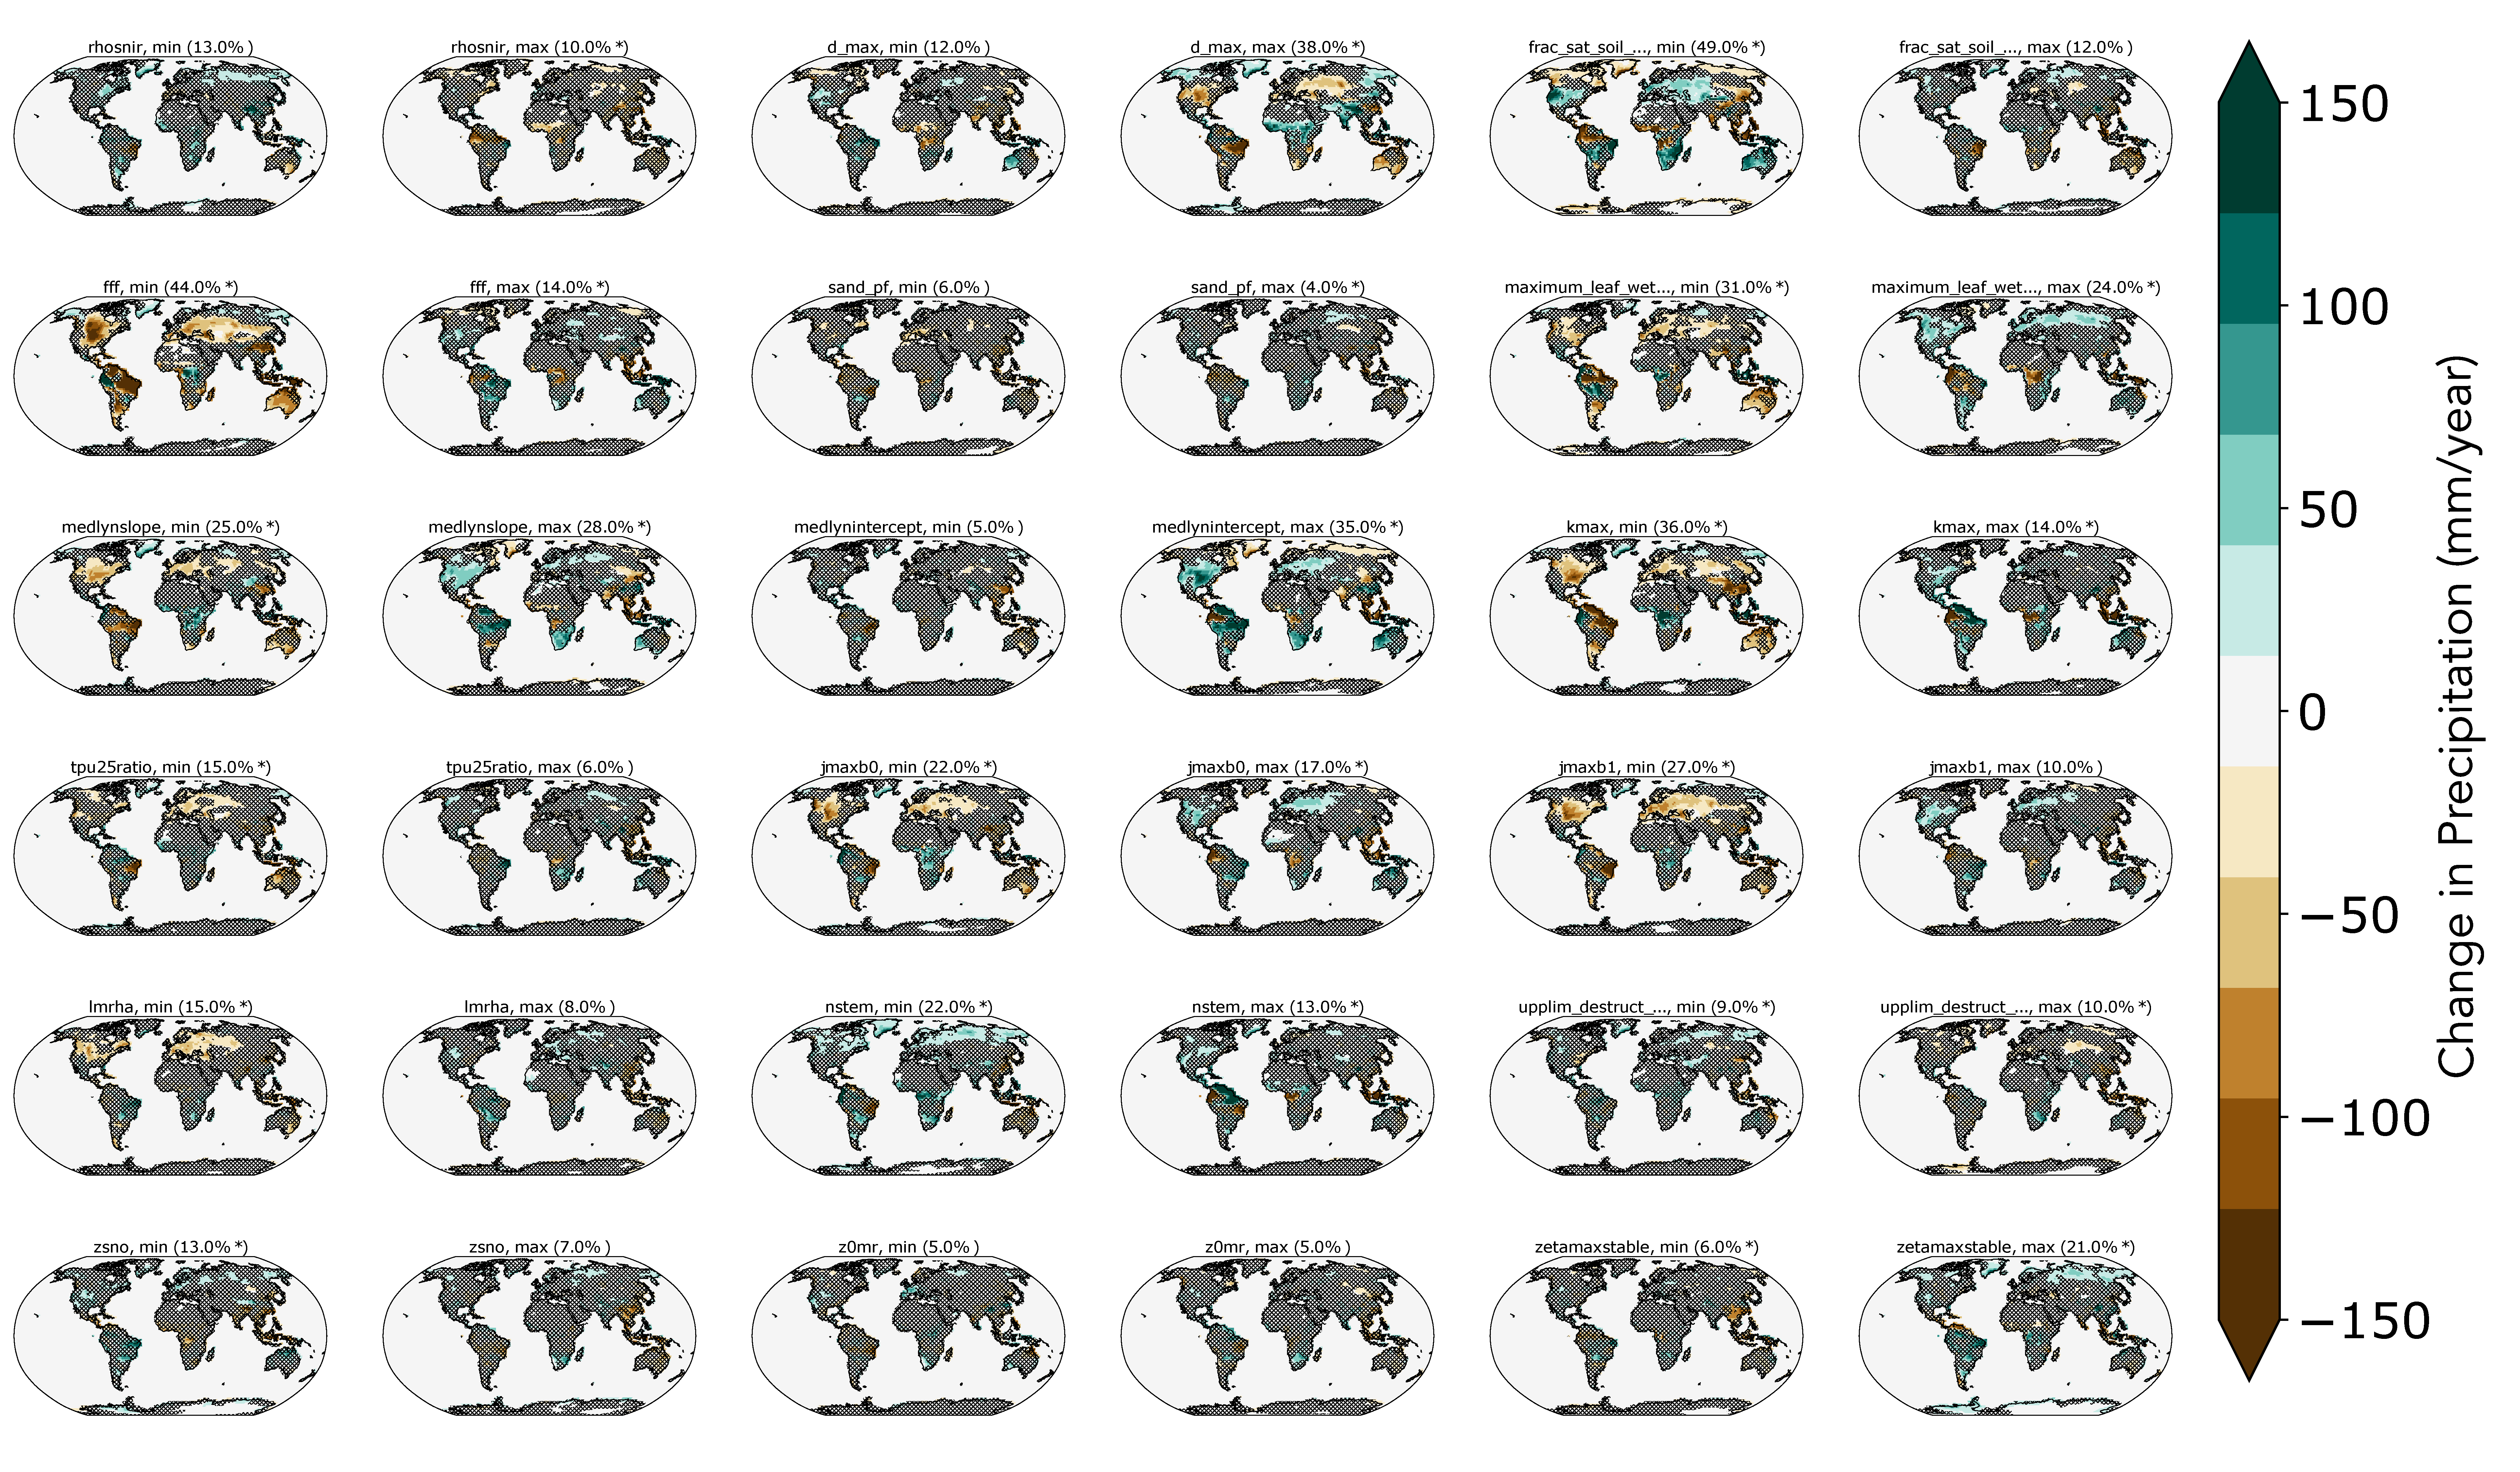
\includegraphics[width=\textwidth]{writing/figs/Figure_S7.pdf}
\caption{Maps of annual mean land precipitation changes for each ensemble member, compared to the reference case with default parameterizations. Hatching indicates regions where the precipitation change was insignificant at the 0.05 significance level. The percentage of land with statistically significant temperature changes are shown in parentheses, and * indicates field significance.For each grid cell, we performed a two-tailed Student’s t-test to test whether the ensemble member mean (standard deviation calculated from the distribution from interannual variability in the ensemble member mean) was different from the default mean (standard deviation calculated from the distribution from interannual variability in the default mean). We test for field significance using Walker’s test.}
\label{fig:supp_maps_precip}
\end{figure}

\begin{figure}[htb!]
\noindent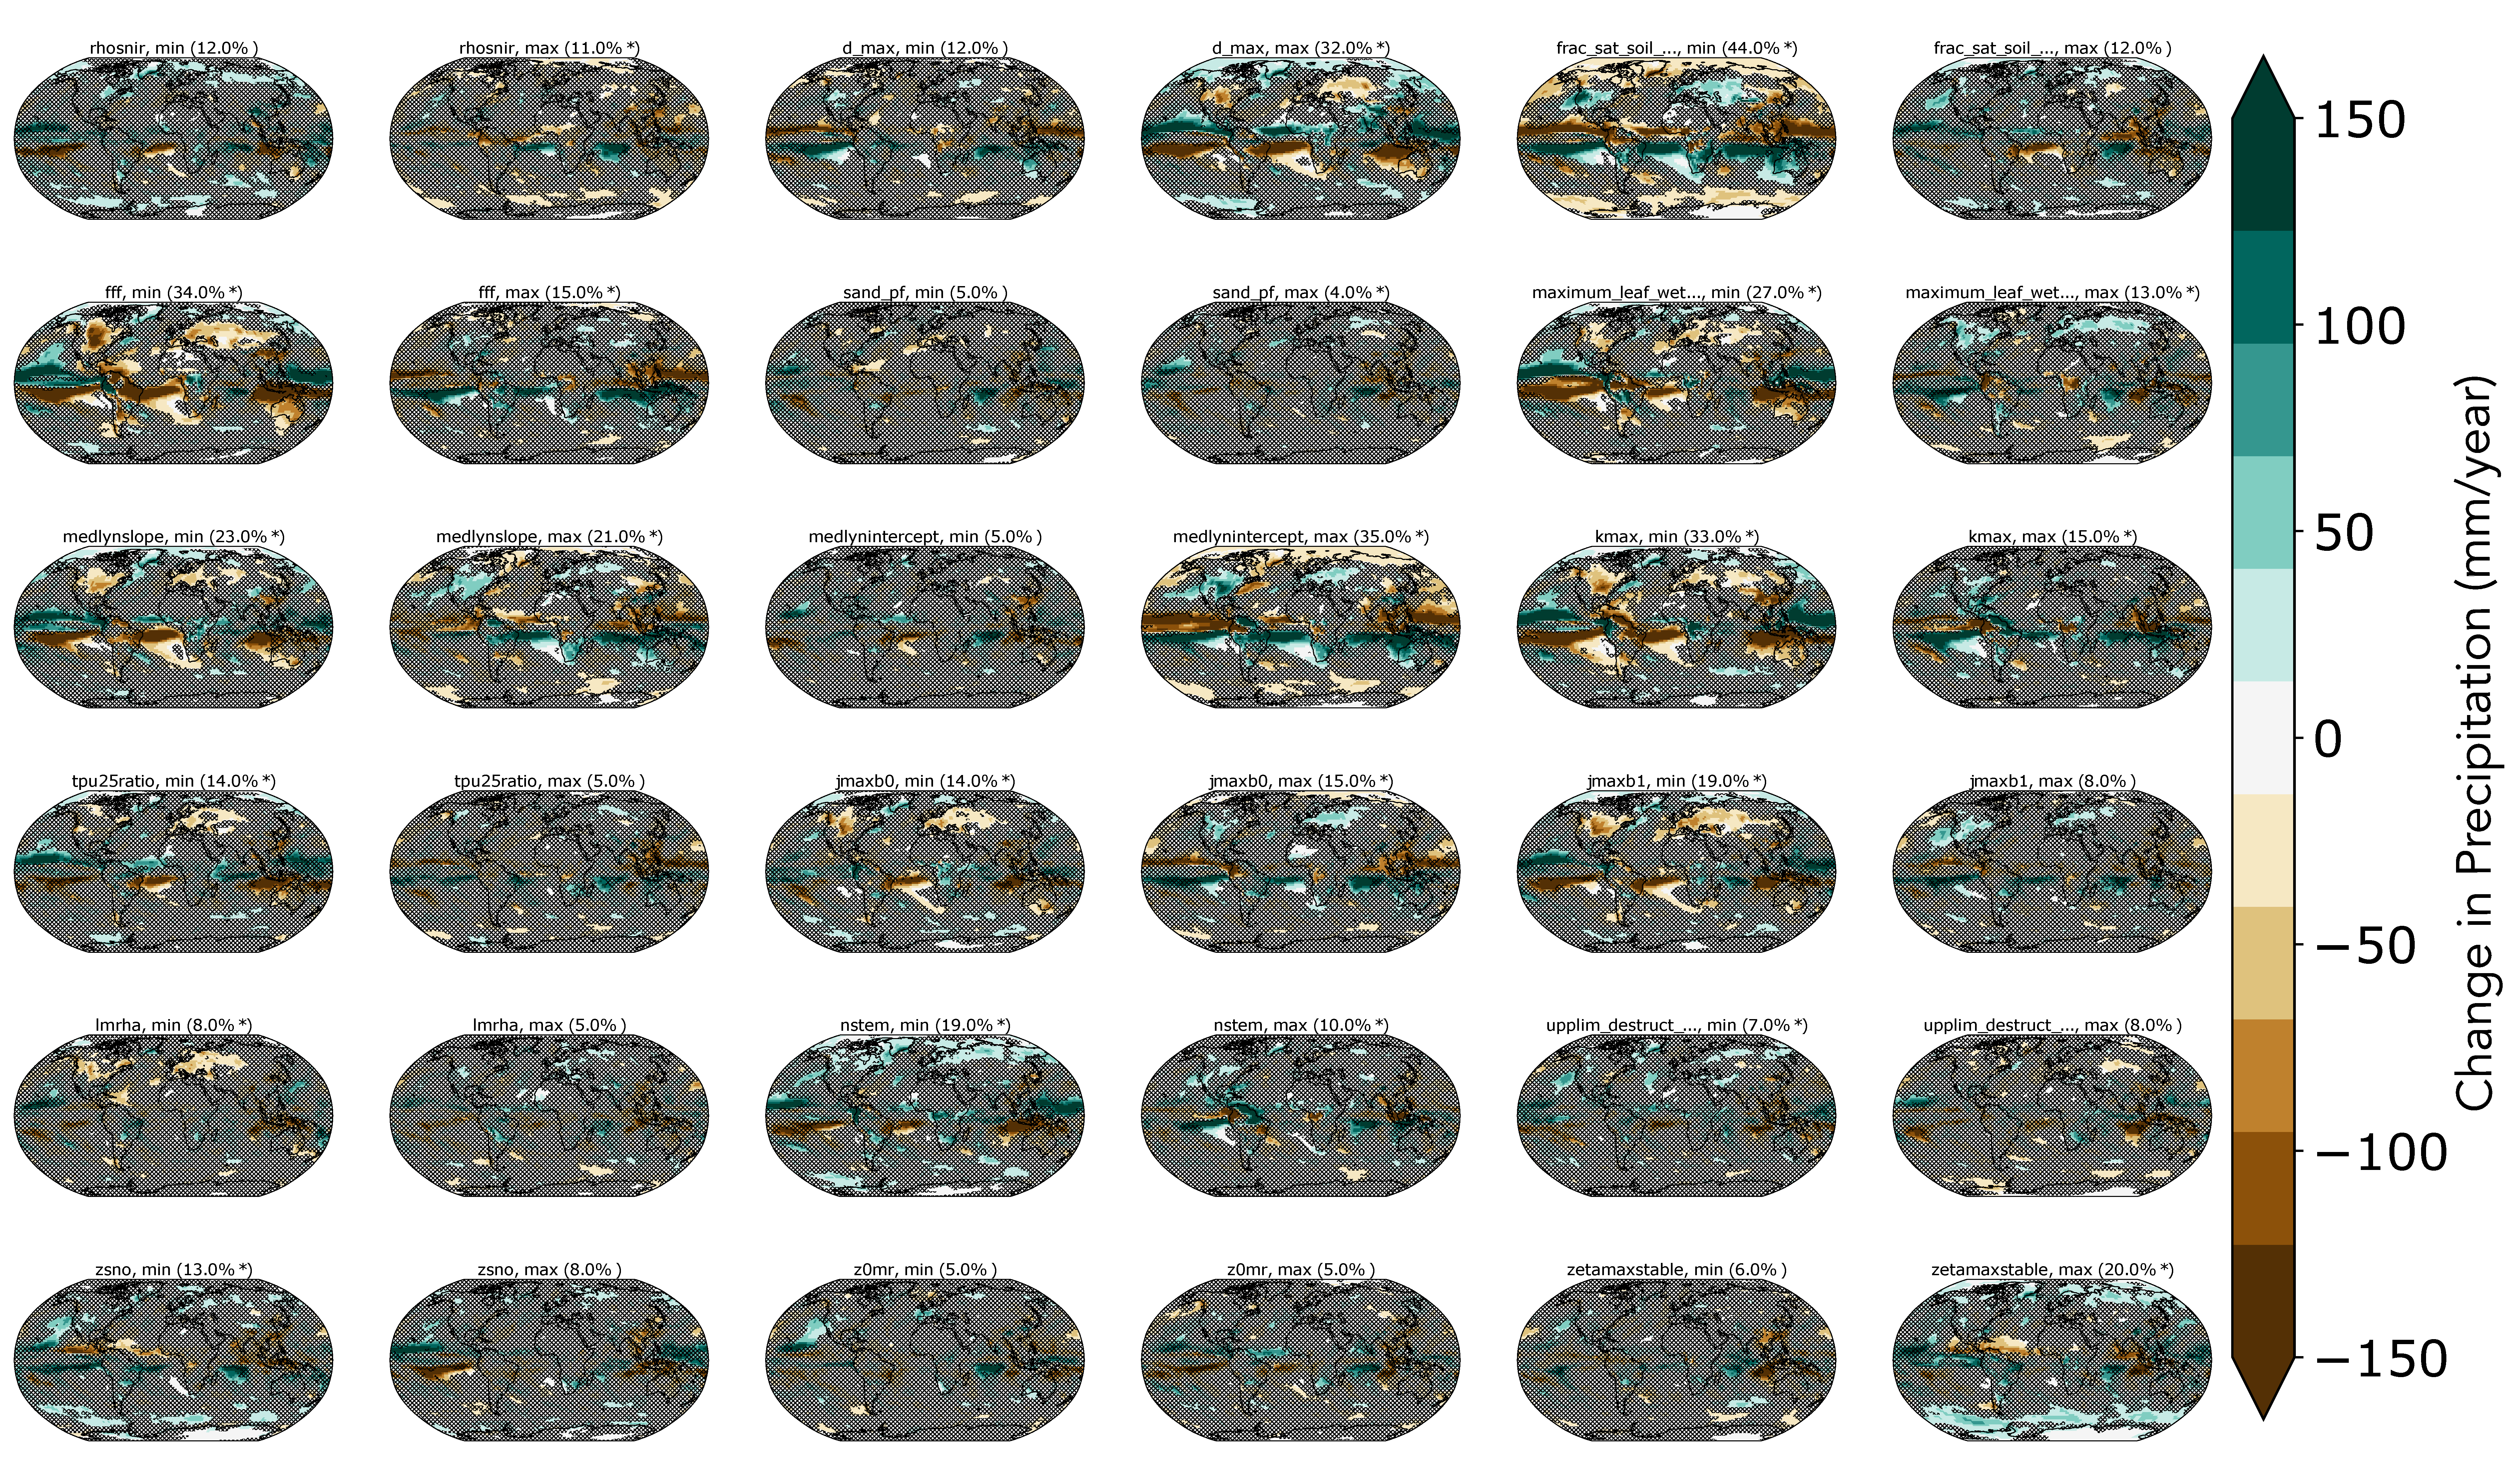
\includegraphics[width=\textwidth]{writing/figs/Figure_S7_withOcean.pdf}
\caption{Maps of annual mean precipitation changes for each ensemble member, including both land and ocean. Hatching and significance testing is as in Figure S7, but the title indicates the total percentage of the Earth surface (including land and ocean) with statistically significant temperature changes.}
\label{fig:supp_maps_precip_landAndOcean}
\end{figure}

\begin{figure}[htb!]
\noindent\includegraphics[width=\textwidth]{writing/figs/Figure_S8.pdf}
\caption{Percentage of land area with statistically significant temperature vs. precipitation changes for each ensemble member in the PPE. Ensemble members are colored by parameter category, as in Figure 1. Zetamaxstable is indicated with a filled circle because it is a frequent outlier.}
\label{fig:supp_pct_stat_sig_land}
\end{figure}

\begin{figure}[htb!]
\noindent\includegraphics[width=\textwidth]{writing/figs/Figure_S9_Percentage_Significant_Sign_Change.pdf}
\caption{Sign of change of statistically significant mean climate changes across the PPE. Percent of land area experiencing statistically significant decreases vs. increases in temperature (left) and precipitation (right) for each PPE ensemble member. Ensemble members are colored by parameter category, as in Figure 1. Zetamaxstable is indicated with a filled circle because it is a frequent outlier.}
\label{fig:supp_pct_stat_sig}
\end{figure}

\begin{figure}[htb!]
\noindent\includegraphics[width=\textwidth]{writing/figs/Figure_S_Precip_Change_Significance_by_Parameter.pdf}
\caption{Percentage of global land area that experiences statistically significant changes in annual mean precipitation due to perturbations in each parameter. For each land grid cell, we performed a two-tailed Student’s t-test to test whether the parameter maximum simulation was different from the parameter minimum simulation.}
\label{fig:supp_precip_significance_changes}
\end{figure}

\begin{figure}[htb!]
\noindent\includegraphics[width=\textwidth]{writing/figs/PRECT_range_absolute_change.pdf}
\caption{Range in annual mean precipitation changes across the PPE, on an absolute basis (left) and as a percentage of the default precipitation (right). Hatching indicates regions where annual mean precipitation changes were statistically insignificant for five or more ensemble members.
}
\label{fig:supp_precip_range}
\end{figure}

\begin{figure}[htb!]
\noindent\includegraphics[width=\textwidth]
{writing/figs/Figure_S_Minimal_RESTOM_differences.pdf}
\caption{Time series of the net radiative flux at the top of the model (RESTOM), as calculated from the net solar flux at top of model (FSNT) minus the net longwave flux at top of model (FLNT). The average RESTOM for the last 100 years of the reference case is -0.15 W$/$m$^2$. RESTOM varied minimally across the ensemble ($\sigma$=0.010 W/m$^2$), and was not statistically significantly different from the reference case for any ensemble member. Significance was tested using two-tailed Student’s t-test on the  time series of annual mean RESTOM.}
\label{fig:supp_TOA_energy_balance}
\end{figure}

\begin{figure}[htb!]
\noindent\includegraphics[width=\textwidth]{writing/figs/placeholder.pdf}
\caption{Spin up. fast atmospheric processes, leaf area, soil moisture and temperature, and the surface ocean to equilibrate. [Add supplemental figure showing the spin up period]}
\label{fig:supp_spinup}
\end{figure}

%\captionsetup[table]{format=cancaption,labelformat=cancaptionlabel}
 \begin{table}[htb!]
 \centering
\noindent\includegraphics[width=0.5\textwidth]{writing/figs/Table_Land2Atm_Quantities.pdf}
  \caption{Quantities that the land model passes to the atmosphere in CESM2. \\
  \footnotesize{*Note that net ecosystem exchange does not impact the atmosphere in our experimental design because our experimental design held atmospheric CO$_2$ concentrations fixed.}}
 \label{table:metrics_of_impact}
 \end{table}



\begin{table}[htb!]
\noindent\includegraphics[width=\textwidth]{writing/figs/Table_Quantities_Used_In_Parameter_Selection.pdf}
  \caption{Metrics for evaluating parameter impact on land-to-atmosphere fluxes. \\
    \footnotesize{*TK Land atmosphere coupling
    }}
 \label{table:land2atm_fluxes}
 \end{table}

\begin{sidewaystable}[htb!]
\noindent\includegraphics[width=\textwidth]{writing/figs/Table_Parameter_List.pdf}
  \caption{Land parameters used in this study.\\
    \footnotesize{$^1$TK Note about parameter ranges
    }}
 \label{table:param_list}
 \end{sidewaystable}
\end{document}